\documentclass{article}
\usepackage[utf8]{inputenc}

\title{Project 2: Trading with ETF II}
\author{Roar Nind Steffensen (s144107)}
\date{November 2015}

\usepackage{natbib}
\usepackage{graphicx}
\usepackage{geometry}
\usepackage{subcaption}
 \geometry{
 a4paper,
 total={150mm,237mm},
 left=30mm,
 top=30mm,
 }

\begin{document}

\maketitle

\section{Analysis of 4 selected ETFs}
\subsection{Data analysis}
By looking at the data from the previous project, we can now calculate the geometric mean, the relative weekly return percentage and the volatility. 
\\
The geometric mean is found by 
\begin{equation} \label{aweek}
a_{week}=\sqrt[454]{a}=\mathbf{exp}\left( \frac{1}{454}\cdot \sum_{t=1}^{454} \textbf{log}(a_t)\right)
\end{equation}
With $a_t$ beeing the projection factor for the \textit{t}'th week. And the relative weekly returns (in percentage) are found by

\begin{equation} \label{rweek}
r_{week} = (a_{week}-1)\cdot100\%
\end{equation}
\\
In addition we find the volatility, which is a tool for the risk you take by betting on one of the ETFs. This is calculated by

\begin{equation}\label{volatility}
v=100\cdot\sqrt{\frac{1}{454}\cdot\sum_{t=1}^{454}(a_t-\bar{a})^2} 
\end{equation}

Where $\bar{a}$ is the mean of the projection factor.
\\ 
This is done for each of the four selected ETFs and is shown in Table \ref{Tabel_ETF_GM_r}

\begin{table}[h!]
\centering
\caption{Data analysis ETFs} \vspace{1mm}
\label{Tabel_ETF_GM_r}
\begin{tabular}{|c|c|c|c|}
\hline
    & \begin{tabular}[c]{@{}c@{}}Geometric\\ mean\end{tabular} & \begin{tabular}[c]{@{}c@{}}Relative weekly\\ return (Pct)\end{tabular} & Volatility (Pct)\\ \hline
AGG & 1.000248  & 0.02479365  & 0.5975841 \\ \hline
VAW & 1.001133  & 0.11334644  & 3.608286 \\ \hline
IWN & 1.000668  & 0.06684908  & 3.201547 \\ \hline
SPY & 1.001049  & 0.10490378  & 2.478601 \\ \hline
\end{tabular}
\end{table}

In this project we work with specific numerical variables, where the most essential variables are as follows:
\\ 
\subsection{Important Varibles}
- \textbf{Geo.mean}

This stands for the \textit{Geometric mean relative weekly return} denoted $r_{week}$. From Eq. \ref{rweek} and \ref{aweek} wee see that $r_{week}$ depends on the geometric mean. The geometric mean, also called the average projection factor per period (week in our case), expresses the average change in exchange rate per period. Another way of saying it, is that the projection factor describes relative difference in exchange rate from one week to the other, so the average projection factor per period / geometric mean, as the name states, is an average of the relative difference over each period. This means that $r_{week}$ is the average relative return per week. \\
\\
- \textbf{VaR}

This stands for \textit{Value at Risk} and is a measure for how much an ETF can drop in value during one period within a certain probability, knowing that it is impossible to asses the maximum since it is unknown. This is based on historical data assuming that the risk for the future period (week) follows the model based on data gathered before that period. \\
\\
- \textbf{Volatility}

This stands for \textit{The weekly volatility} denoted $v$.  From Eq. \ref{volatility} we  see that it's a tool for the standard deviation on the projection factor, and is therefore a description of how rapid a change in return there is.\\

\subsection{Variable correlation}
The variables are correlated and it is therefore reasonable to look at the correlation of the given variables to check the linear relationship between the variables. We will try and look at the correlatiuon between \textit{Geo.mean} and \textit{maxTuW}.\\

The correlation coefficient $r$ is given by
\begin{equation}\label{covariance}
r=\frac{1}{n-1}\sum_{i=1}^{n}\left(\frac{x_i-\bar{x}}{s_x}\right)\left(\frac{y_i-\bar{y}}{s_y}\right)= \frac{s_{xy}}{s_x\cdot s_y}
\end{equation}
\\
Where $n$ is the size of our samples (they must be of equal length), $x_i$ is the $i$'th component of sample $x$, $\bar{x}$ is the mean of sample $x$ and $s_x$ is the standard deviation for sample $x$, (likewise for $y_i, \bar{y}, s_y$) and $s_{xy}$ is the covariance between the two samples.\\

If we insert the data from our ETFs with $n = 95-4=91$ 

\begin{equation}\label{covariance_w.data}
r=\frac{1}{91-1}\sum_{i=1}^{91}\left(\frac{Gm_i-0.076879}{0.082313}\right)\left(\frac{mTW_i-306.60}{43.5428}\right)=-0.21761
\end{equation}

This correlation coefficient states that since the value is negative, it means that they have a negative "feedback" on each other and since it is a small value that they are not highly correlated. By using the code in R we get the correlations for all the variables as seen in Tabel \ref{correlations}, and with further investigation we see that our found value for $r$ is correct.

\begin{table}[h!]
\centering
\caption{Correlations between variables} \vspace{1mm}
\label{correlations}
\begin{tabular}{|c||c|c|c|c|c|c|}
\hline
           & Geo.mean   & Volatility & maxDD      & maxTuW     & VaR        & CVaR       \\ \hline \hline
Geo.mean   & 1.0000  & -0.3973 & -0.4480 & -0.2176 & 0.4486  & 0.4265  \\ \hline
Volatility & -0.3973 & 1.0000  & 0.8693  & 0.2768  & -0.9714 & -0.9915 \\ \hline
maxDD      & -0.4480 & 0.8693  & 1.0000  & 0.3148  & -0.8527 & -0.9013 \\ \hline
maxTuW     & -0.2176 & 0.2768  & 0.3148  & 1.0000  & -0.2921 & -0.2906 \\ \hline
VaR        & 0.4486  & -0.9714 & -0.8527 & -0.2921 & 1.0000  & 0.9652  \\ \hline
CVaR       & 0.4265  & -0.9915 & -0.9013 & -0.2906 & 0.9652  & 1.0000  \\ \hline
\end{tabular}
\end{table}

To get a more visual perspektive on the correlation, we plot the variables vs each others, and see their relationsship. If this is done we expect especially the Volatility and CVaR to be very linear inverse proportional to each other since the correlation coefficient is strongly negative ( the limits of $r$ is -1 an 1) .\\

\begin{figure}[h!]
\centering
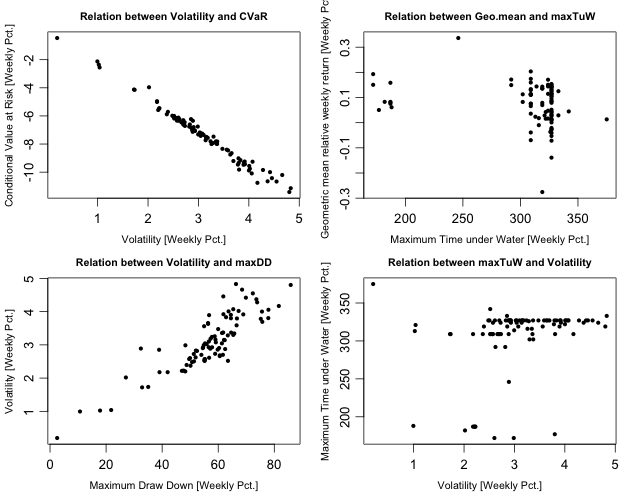
\includegraphics[width=\textwidth]{fig/Rplot.png}
\caption{Variable relationships}
\label{fig:4p}
\end{figure}


As expected, if we look at Figure \ref{fig:4p} we see that the top left graph showing CVaR as a function of Volatility, and that it resembles a straight line with inverse proportionality. 

\subsection{Linear fit and error analysis}
If we were to formulate model of a linear regression, with \textit{Geo.mean} as the dependent variable $Y_i$ and VaR as the explanatory variable $x_i$, we get: 

\begin{equation}
Y_i = \hat{\beta_0}+\hat{\beta_1} x_i + \epsilon_i , \hspace{7 mm} i=\{1,...,n\}
\end{equation}

\vspace{2mm}
Where $\beta_0$ and $\beta_1$ is chosen to minimize $\epsilon_i$ and in the case of the correlation between $Y$ and $x$ is 1 og -1, $\epsilon$ would be zero, meaning a perfect fit. The reason for \textit{VaR} as the explanatory variable is that we want the absolute value of the correlation to be as near 1 as possible in order to minimize $\epsilon$, and except for \textit{Geo.mean}'s correlation with itself, which of course gives a straight line, \textit{VaR} has has the highest correlation with \textit{Geo.mean}. \\

For this choice of variables we can find the $\beta_0$ and $\beta_1$ parameters using least square method. 

\begin{equation}\label{beta1}
\hat{\beta_1}=
    \frac
        {\sum_{i=1}^n\left(Y_i-\bar{Y}\right)\left(x_i-\bar{x}\right)}
        {\sum_{i=1}^n\left(x_i-\bar{x}\right)^2}
\end{equation}

\begin{equation}\label{beta0}
\hat{\beta_0}=
    \bar{Y}-\beta_1 \bar{x}
\end{equation} \\
\\

By inserting the our data in Eq. \ref{beta1} and \ref{beta0} we get

\begin{equation}\label{beta1}
\hat{\beta_1}=
    \frac
        {\sum_{i=1}^n\left(Gm_i-0.07687915\right)\left(VaR_i-(-4.696756)\right)}
        {\sum_{i=1}^n\left(VaR_i-(-4.696756)\right)^2}
        =0.02666589
\end{equation}

\begin{equation}\label{beta0}
\hat{\beta_0}=
    0.07687915-0.02666589 \cdot (-4.696756)
    =0.2021223
\end{equation}
\\

Meaning we have an intersection at 0.2 and a slope of 0.026 in our linear fit. This means that our \textit{Geo.mean} is estimated to 0.2 when \textit{VaR} is zero, and is slightly raised when \textit{VaR} rises. Here it might be reasonable to look at the variance of the errors $\sigma^2$

\begin{equation}
\sigma^2=
    \frac
        {\sum_{i=1}^n \epsilon_i^2}
        {n-2} 
    =
    \frac
        {\sum_{i=1}^n \left(Y_i-\left(\beta_0+\beta_1 \bar{x}\right)\right)^2}
        {n-2}
\end{equation}
Which gives us 

\begin{equation}
\sigma^2=
    \frac
        {\sum_{i=1}^{91} \left(Gm_i-\left(0.2021223 +0.02666589 
        \cdot( -4.696756)\right)\right)^2}
        {91-2}=0.005472976
\end{equation}

By comparing with the direct R-command on Figure \ref{fig:Rcode_lm} we see that our calculations match (noting that the "Residual standard error" is the square root of the variance of the errors). 

\begin{figure}[h!]
\centering
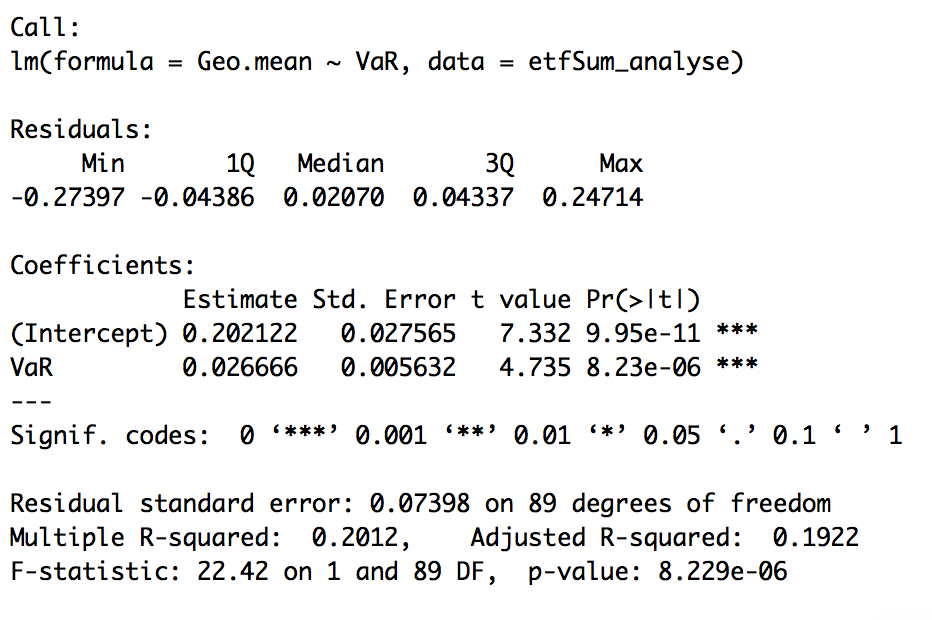
\includegraphics[width=0.7\textwidth]{fig/lm.png}
\caption{R-command values for linear fit parameters and error}
\label{fig:Rcode_lm}
\end{figure}

So we have found the estimates of our linear coefficients and from the R-command values we see the standard deviations of these coefficients, which are around 15\% of their actual values meaning this is a quite bad linear fit. We got an estimate of our standard deviation of the errors (the square root of our variation of errors) which represents the range where 68\% of the errors are within. Which is calculated by using $n-2$ degrees of freedom. The reason for this is that we need at least three data points before we get any usable result (though with three points it would be bad), otherwise the line would follow the two data points perfectly. And when speaking of the variance we have our $R^2$ which is essentially the area of the squares with side lengths from our points to our linear fit. The reason it is squared is so all values drag the error in the same direction, so that a positive error and a negative error would not cancel each other out. \\

Before we accept our coefficients and linear fit we have to justify that our assumption of the residuals is following the normal distribution, this can be done by analyzing the relationship between the residuals, the fitted parameters and our samples. Finally checking our residuals with the qq-plot to check for normal behavior. This is done in Figure \ref{fig:normal_check}. To justify our assumptions there must be no systematical behavior between residuals, the fitted parameters, but a nice linear fit for the qq-plot, and in Figure \ref{fig:normal_check} we see that this is the case. Our assumption is then justified. 

\begin{figure}[h!]
\centering
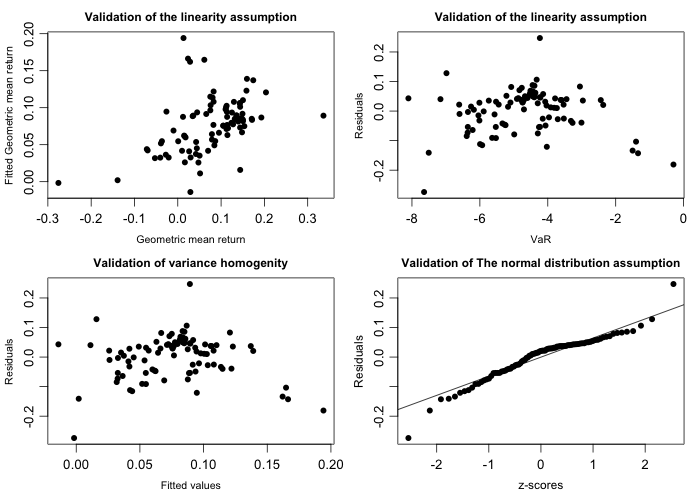
\includegraphics[width=\textwidth]{fig/normal_check.png}
\caption{Checking for normal behavior}
\label{fig:normal_check}
\end{figure}

Once we have our coefficients set we can find the 95\% confidence intervals.

\begin{equation}\label{beta0_int}
\beta_0 \in \hat{\beta_0} \pm t_{1-\alpha/2} \; \hat{\sigma}_{\beta_0}
\end{equation}
\begin{equation}\label{beta1_int}
\beta_1 \in \hat{\beta_1} \pm t_{1-\alpha/2} \; \hat{\sigma}_{\beta_1}
\end{equation}

With $t_{1-\alpha/2}$ being the ($1-\alpha/2$) quartile from the t-distribution with $n-2$ degrees of freedom, which gives us $t_{1-\alpha/2}=1.986979$. Practically this is only the right tail of the distribution, but the left tail is simply the negative value of the right tail because of symmetry. Before we can calculate the intervals, we need to find $\hat{\sigma}_{\beta_0}$ and $\hat{\sigma}_{\beta_1}$ 

\begin{equation}
\hat{\sigma}_{\beta_0}=
                \hat{\sigma}\sqrt{\frac{1}{n} + 
                \frac{\bar{x}^2}{\sum_{i=1}^n (x_i-\bar{x})^2}} ; \hspace{5mm}
\hat{\sigma}_{\beta_1}=
                \hat{\sigma}\sqrt{
                \frac{1}{\sum_{i=1}^n (x_i-\bar{x})^2}}
\end{equation}
\\

Inserting our data gives us 

\begin{equation}
\hat{\sigma}_{\beta_0}=
                0.07397956\sqrt{\frac{1}{91} + 
                \frac{(-4.696756)^2}{\sum_{i=1}^{91} (VaR_i-(-4.696756))^2}}
                =0.02756548
\end{equation}

\begin{equation}
\hat{\sigma}_{\beta_1}=
                0.07397956\sqrt{
                \frac{1}{\sum_{i=1}^{91} (VaR_i-(-4.696756))^2}}
                =0.005631991
\end{equation}
\\

Inserting this in Eq. \ref{beta0_int} and \ref{beta1_int} we get

\begin{equation}\label{beta0_int}
\beta_0 \in 0.2021223 \pm 1.98697 \cdot 0.02756548
        \in \{ 0.1473503 ; 0.2568943\}
\end{equation}
\begin{equation}\label{beta1_int}
\beta_1 \in 0.02666589 \pm 1.98697 \cdot 0.005631991
        \in \{0.01547524; 0.03785653 \}
\end{equation}
\vspace{2mm}
\\

And by checking our results with the direct R-command in Figure \ref{fig:Rcode_int} we see that our calculations are correct.

\begin{figure}[h!]
\centering
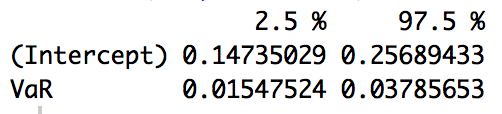
\includegraphics[width=6cm]{fig/Rcode_int.png}
\caption{Direct R-command values for 95\%confidence interval}
\label{fig:Rcode_int}
\end{figure}

Testing this with our R-code we can see the relationship between \textit{Geo.mean} and \textit{VaR} with the confidence interval of 95\%. This can be seen in Figure \ref{fig:CInt}.

\begin{figure}[h!]
\centering
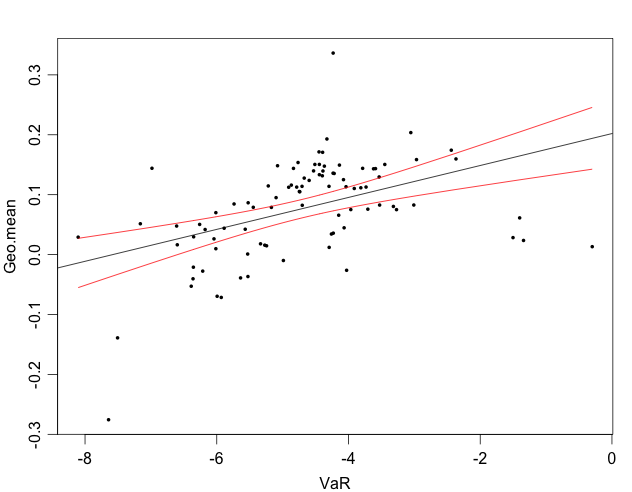
\includegraphics[width=0.6\textwidth]{fig/CInt.png}
\caption{Geo.mean and VaR relationship with confidence intervals }
\label{fig:CInt}
\end{figure}

Now we can see that our linear fit/model is quite reasonable but still holds quite an uncertainty, the significans of the contribution to the dependent variable from the explanatory variable can be tested with a hypothesis. In this hypothesis we do not care for the intercept; we are interested in the slope. If we state a null hypothesis for the slope coefficient $\beta_1$ we can check if $\beta_1$ has no dependence, which concludes that our fit has no meaning / unusable information. \\

The hypothesis is setup as follows:

\begin{equation}
H_{01}: \beta_1 =1 ; \hspace{4mm} H_{11}: \beta_1 \neq 1
\end{equation}

First we must find our $t_{obs}$ for the $\beta_1$: 

\begin{equation}
T_{\beta_1}=\frac{\hat{\beta_1}-\beta_{0,1}}{\hat{\sigma}_{\beta_1}} = \frac{0.02666589}{0.005631991}=4.734717
\end{equation}  

Giving us our p-value of $8.229448e-06$ meaning our $H_{01}$ is rejected, meaning we can not deny a dependence between \textit{Geo.mean} and \textit{VaR}, the calculations are confirmed as seen on Figure \ref{fig:Rcode_lm} under "t value" and "Pr(\textgreater \textbar t\textbar)". 

Since our model holds valid information of the \textit{Geo.mean} vs. \textit{VaR} we want to find the prediction interval.

\begin{equation}
{y}_{new} \in
\hat{\beta}_0+\hat{\beta}_1 x_{new} \pm 
t_{1-\alpha/2} \; \hat{\sigma}
\sqrt{
    1+\frac{1}{n}+ \frac{(x_{new}-\bar{x})^2}{S_{xx}}
    }
\end{equation}

The difference here, is that we always have a full standard deviation as an uncertainty compared to the confidence intervals for the linear fit as seen on Figure \ref{fig:CPInt}. 

\begin{figure}[h!]
\centering
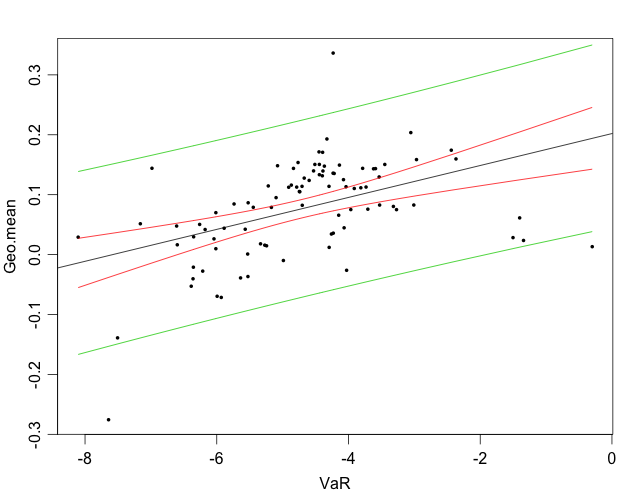
\includegraphics[width=0.8\textwidth]{fig/CPInt.png}
\caption{Confidence intervals (red) and prediction intervals (green)}
\label{fig:CPInt}
\end{figure}

If we look at the prediction intervals for our previous selected ETFs from project 1 we get the following predictions.\\

\textit{Geo.mean} prediction for SPY ETF:
    \begin{equation}
    {SPY}_{Gm} \in
    0.2021+0.02667\cdot SPY_{VaR} \pm
    1.987 \cdot 0.07398
    \sqrt{
    1+\frac{1}{91}+ \frac{(SPY_{VaR}-(-4.697))^2}{172.5}
    }
    \end{equation}
    
    \begin{equation}
    SPY_{Gm} \in \{ -0.04480496 ; 0.25163548 \}
    \end{equation}\\

\textit{Geo.mean} prediction for IWN ETF:
    \begin{equation}
    {IWN}_{Gm} \in
    0.2021+0.02667\cdot IWN_{VaR} \pm
    1.987 \cdot 0.07398
    \sqrt{
    1+\frac{1}{91}+ \frac{(IWN_{VaR}-(-4.697))^2}{172.5}
    }
    \end{equation}
    
    \begin{equation}
    IWN_{Gm} \in \{ -0.07455842 ; 0.22105983 \}
    \end{equation}\\

\textit{Geo.mean} prediction for AGG ETF:
    \begin{equation}
    {AGG}_{Gm} \in
    0.2021+0.02667\cdot AGG_{VaR} \pm
    1.987 \cdot 0.07398
    \sqrt{
    1+\frac{1}{91}+ \frac{(AGG_{VaR}-(-4.697))^2}{172.5}
    }
    \end{equation}
    
    \begin{equation}
    AGG_{Gm} \in \{ 0.0227774 ; 0.3299464 \}
    \end{equation}\\
    
\textit{Geo.mean} prediction for VAW ETF:
    \begin{equation}
    {VAW}_{Gm} \in
    0.2021+0.02667\cdot VAW_{VaR} \pm
    1.987 \cdot 0.07398
    \sqrt{
    1+\frac{1}{91}+ \frac{(VAW_{VaR}-(-4.697))^2}{172.5}
    }
    \end{equation}
    
    \begin{equation}
    VAW_{Gm} \in \{ -0.0864599 ; 0.2094250 \}
    \end{equation}\\
\\
Which matches the results from the direct R-command as seen on Figure \ref{fig:Rcode_PInt}

\begin{figure}[h!]
\centering
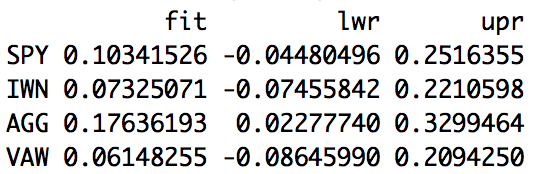
\includegraphics[width=6cm]{fig/Rcode_PInt.png}
\caption{Prediction intervals from direct R-command}
\label{fig:Rcode_PInt}
\end{figure}

And if we check the intervals for our four ETFs with the calculated \textit{Geo.mean} values from Table \ref{correlations} with the \textit{VaR} values from Figure \ref{RiskTable}, we see that they are well within our prediction intervals which approves that our ability to predict is valid within a certain interval (as long as we stay within the range of our data). \\

\begin{figure}[h!]
\centering
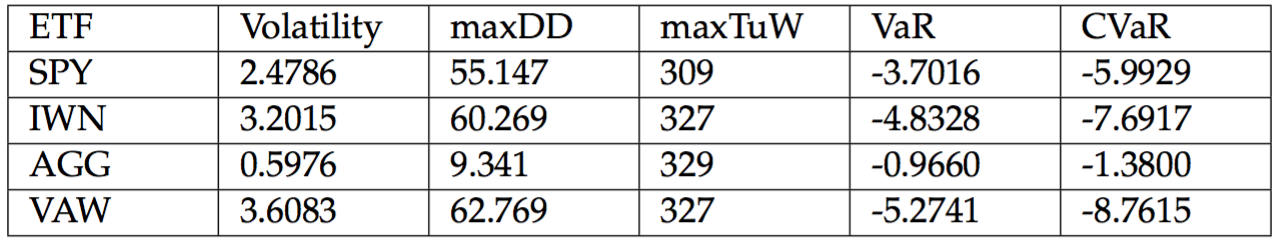
\includegraphics[width=0.7\textwidth]{fig/RiskTable.png}
\caption{Risk measure values for the four ETFs.}
\label{RiskTable}
\end{figure}

Now, there is still a perspective we have not tackled. What about the correlation between \textit{VaR} and the \textit{Volatility}? how does this effect our system? It might be, that our \textit{Geo.mean} is only properly modelled if both are taken account for. This can be checked in the data from R seen in Figure \ref{fig:Rcode_lm}, \ref{fig:subim1} and \ref{fig:subim2}. 

\begin{figure}[h!]
\begin{subfigure}{0.5\textwidth}
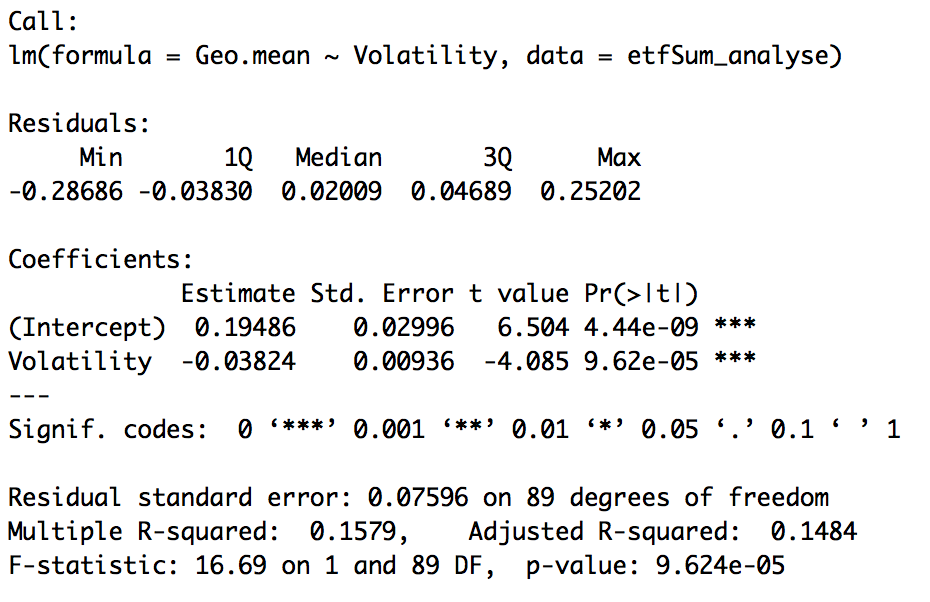
\includegraphics[width=0.9\linewidth]{fig/lmGmVo} 
\caption{Geo.mean vs Volatility linear fit}
\label{fig:subim1}
\end{subfigure}
\hfill
\begin{subfigure}{0.5\textwidth}
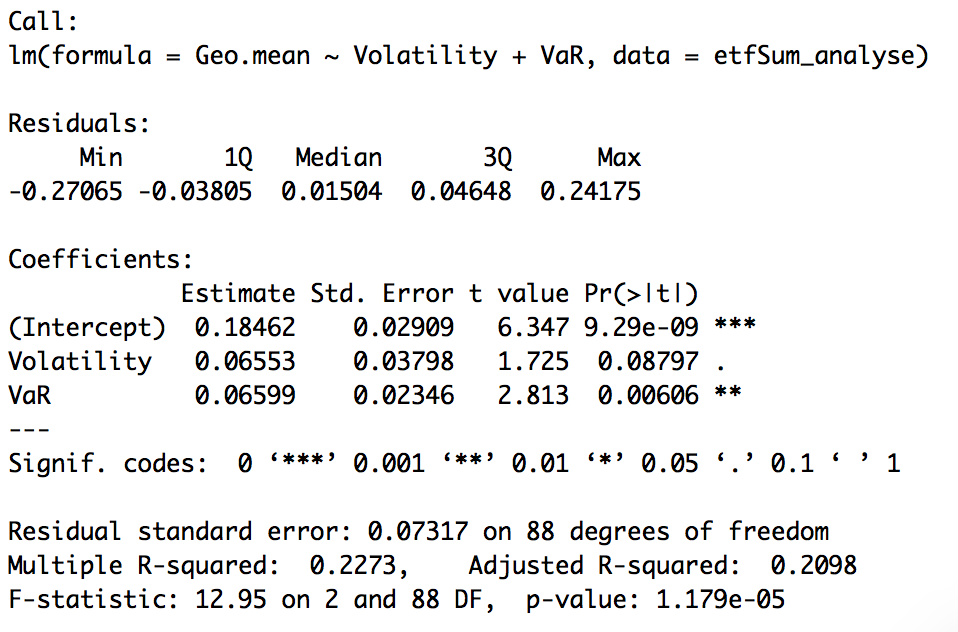
\includegraphics[width=0.9\linewidth]{fig/lmGmVarVo}
\caption{Geo.mean vs Volatility + VaR linear fit}
\label{fig:subim2}
\end{subfigure}
\caption{Data for comparison of collinearity}
\label{fig:Data}
\end{figure}

Now as seen in the data from our R-code, we see that the estimates for our \textit{VaR} coefficient $\hat{\beta}_1$ differs with a factor of 2.5 which is a rather big change, meaning it is not very stable, and we also see that the \textit{Volatility} coefficient changes sign meaning that the two explanatory variables has an influence on each other when both are drawn into our model. So is our precious model disproved? If we look towards Figure \ref{fig:subim2} we see that the p-value for our \textit{Volatility} is 0.09 meaning that it can be removed from our model, meaning that even though the \textit{Geo.mean} is dependent on the \textit{Volatility} (as seen in Figure \ref{fig:subim1} with a p-value of 9.6e-5), when we have both the \textit{VaR} and \textit{Volatility} in perspective, the correlation between our explanatory variables makes the \textit{Volatility} less important. So the interpretation of the explanatory variables effect on the dependent variable changes. \\

Collinearity is an important aspect when looking at statistic models, since we wish to compute a model as precise as possible. There can be dramatic differences between several individual models of a dependant variable and several explanatory variables, and one combined model caused by the collinearity effect between the explanatory variables. When one inspects such a problem, it is practical to check the fully combined model
and then analyze the different null hypothesis' for each variable and check for their relevance. 







\end{document}
